\documentclass[11pt,a4paper]{article}
\usepackage[T1]{fontenc}
\usepackage{lmodern}
\usepackage[a4paper,margin=2.4cm]{geometry}
\usepackage{amsmath,amssymb,amsthm}
\usepackage{graphicx}
\usepackage{booktabs}
\usepackage{float}
\usepackage{caption}
\usepackage{microtype}
\usepackage[hidelinks]{hyperref}

\graphicspath{{../results/figures/}}
\captionsetup{font=small,labelfont=bf}
\setlength{\emergencystretch}{2em}
\newtheorem{proposition}{Proposition}
\numberwithin{equation}{section}

\title{Two-Armed Stochastic Bandits\\with Change Points and Noisy Observations}
\author{Xiangyu Luo}
\date{Written solution: 29 September 2026 \quad Numerical study: October 2026}

\begin{document}
\maketitle

\begin{abstract}
A two-armed bandit with two known change points is studied in four steps: a Hoeffding bound for sub-Gaussian means, a UCB algorithm with an $O(\log\tau_1/\Delta)$ high-probability regret bound in the first phase, error bounds for a sliding-window estimator whose window mixes up to three phases, and confidence bounds and budget allocation when every observation carries Laplace noise. Sections~\ref{sec:setting}--\ref{sec:noise} give the written solution. Section~\ref{sec:experiments} adds a reproducible numerical study: it checks every bound by simulation, turns the discussion of part~(c)(iii) into a comparison of window sizes and change-aware variants, and measures how Laplace noise and the allocation of a fixed budget shift the best window. The code is in the accompanying repository (\texttt{src/}); every number in Section~\ref{sec:experiments} is produced by \texttt{src/run\_experiments.py}.
\end{abstract}

\tableofcontents

\section{Problem setting}\label{sec:setting}

Consider a 2-armed stochastic bandit over $T$ rounds. The reward $X_{i,t}$ from arm $i$ at round $t$ is independent and $1$-sub-Gaussian, i.e.
\[
\mathbb E\bigl[e^{\lambda(X_{i,t}-\mu_i(t))}\bigr]\le e^{\lambda^2/2},\qquad \forall\lambda\in\mathbb R,
\]
where $\mu_i(t)$ is the mean of arm $i$ at round $t$. There are two known change points $0<\tau_1<\tau_2<T$, defining three stationary phases:
\[
\mu_i(t)=\begin{cases}\mu_i, & t\le\tau_1,\\ \mu_i', & \tau_1<t\le\tau_2,\\ \mu_i'', & t>\tau_2.\end{cases}
\]
Only arm 1's mean changes at $\tau_1$ (i.e.\ $\mu_2=\mu_2'$), while both arms' means may change at $\tau_2$. Let $\Delta=|\mu_1-\mu_2|$ and $\Delta'=|\mu_1'-\mu_2'|$. Rewards are bounded in $[0,1]$; the width of this range (i.e.\ $1$) is the sensitivity referenced in part~(d).

\section{(a) A Hoeffding-type bound}\label{sec:hoeffding}

\begin{proposition}
For $n$ independent $1$-sub-Gaussian samples with common mean $\mu$, $\mathbb P(|\widehat\mu_n-\mu|\ge t)\le 2\exp(-nt^2/2)$.
\end{proposition}

\begin{proof}
Let $S_n=\sum_{j=1}^n(X_j-\mu)$ and $\widehat\mu_n=n^{-1}\sum_{j=1}^nX_j$. Independence and the sub-Gaussian assumption give, for every $\lambda\in\mathbb R$,
\[
\mathbb E[e^{\lambda S_n}]=\prod_{j=1}^n\mathbb E[e^{\lambda(X_j-\mu)}]\le e^{n\lambda^2/2}.
\]
For a deviation threshold $u>0$ and $\lambda>0$, Markov's inequality yields
\[
\mathbb P(\widehat\mu_n-\mu\ge u)=\mathbb P(e^{\lambda S_n}\ge e^{\lambda nu})\le e^{-\lambda nu}\mathbb E[e^{\lambda S_n}]\le\exp\Bigl(-\lambda nu+\frac{n\lambda^2}{2}\Bigr).
\]
Since $-\lambda nu+n\lambda^2/2=\tfrac n2(\lambda-u)^2-\tfrac{nu^2}2$, choosing $\lambda=u$ gives $\mathbb P(\widehat\mu_n-\mu\ge u)\le e^{-nu^2/2}$. Applying the same argument to $-S_n$ gives $\mathbb P(\widehat\mu_n-\mu\le-u)\le e^{-nu^2/2}$. A union bound therefore proves
\begin{equation}\label{eq:hoeffding}
\mathbb P(|\widehat\mu_n-\mu|\ge u)\le 2e^{-nu^2/2},\qquad u\ge0,
\end{equation}
where the case $u=0$ is immediate.
\end{proof}

\section{(b) UCB in the first phase}\label{sec:ucb}

Let $I_t\in\{1,2\}$ be the selected arm and $N_i(t)=\sum_{s=1}^t\mathbf 1\{I_s=i\}$. The cumulative pseudo-regret is
\[
R(a{:}b)=\sum_{t=a}^b\Bigl(\max_i\mu_i(t)-\mu_{I_t}(t)\Bigr).
\]
Write $H=\tau_1$. For $\Delta>0$, let $i^\star$ and $j$ be the optimal and suboptimal arms in the first phase. Then $\mu_{i^\star}-\mu_j=\Delta$ and $R(1{:}H)=\Delta N_j(H)$. If $\Delta=0$, the pseudo-regret is zero; if $H=1$, it is at most $\Delta$. Assume henceforth that $H\ge2$ and $\Delta>0$.

\paragraph{Concentration at adaptive counts.} Let $(\mathcal F_t)$ be the observation filtration, including the policy's independent randomization, so that $I_t$ is $\mathcal F_{t-1}$-measurable. With $\xi_t=X_{I_t,t}-\mu_{I_t}(t)$, independence implies $\mathbb E[e^{\lambda\xi_t}\mid\mathcal F_{t-1}]\le e^{\lambda^2/2}$. Fix an arm $i$ and deterministic pull indices $a+1,\dots,a+m$. Set
\[
A_s=\mathbf 1\{I_s=i,\ a<N_i(s-1)+1\le a+m\},\qquad C_t=\sum_{s\le t}A_s,\qquad S_t=\sum_{s\le t}A_s\xi_s.
\]
The indicator $A_s$ is predictable, so $\mathbb E[e^{\lambda A_s\xi_s-\lambda^2A_s/2}\mid\mathcal F_{s-1}]\le1$. Hence $M_t(\lambda)=\exp(\lambda S_t-\lambda^2C_t/2)$ is a nonnegative supermartingale with $\mathbb EM_t(\lambda)\le1$. At a deterministic horizon $h$, completion of the block means $C_h=m$. For $u,\lambda>0$, Markov's inequality gives $\mathbb P(C_h=m,\ S_h\ge mu)\le e^{-\lambda mu+m\lambda^2/2}$. Taking $\lambda=u$ and applying the same argument to $-S_h$ gives the completed-block bound
\begin{equation}\label{eq:block}
\mathbb P(C_h=m,\ |S_h|\ge mu)\le 2e^{-mu^2/2}.
\end{equation}

\paragraph{Algorithm.} Fix $\delta\in(0,1)$ and set
\[
L_H=\log\Bigl(\frac{4H}{\delta}\Bigr),\qquad r_H(n)=\sqrt{\frac{2L_H}{n}}.
\]
Pull each arm once. At the start of round $t$, let $\widehat\mu_i(t)=N_i(t-1)^{-1}\sum_{s<t,\,I_s=i}X_{i,s}$. For $3\le t\le H$, choose
\begin{equation}\label{eq:ucb}
I_t\in\arg\max_{i\in\{1,2\}}\bigl\{\widehat\mu_i(t)+r_H(N_i(t-1))\bigr\},
\end{equation}
with arbitrary tie-breaking. The gap $\Delta$ is not needed by the algorithm.

\paragraph{Regret bound.} For each arm and each prefix length $n\le H$, \eqref{eq:block} bounds the probability that the prefix is observed and violates its confidence bound by $2e^{-nr_H(n)^2/2}=2e^{-L_H}=\delta/(2H)$. A union bound over both arms and all $n\le H$ gives an event $\mathcal E_H$ of probability at least $1-\delta$ on which $|\widehat\mu_{i,n}-\mu_i|\le r_H(n)$ for every observed prefix. These bounds therefore hold at the adaptive counts $N_i(t-1)$. On $\mathcal E_H$, selection of the suboptimal arm $j$ at $t>2$ implies
\[
\mu_{i^\star}\le\widehat\mu_{i^\star}(t)+r_H(N_{i^\star}(t-1))\le\widehat\mu_j(t)+r_H(N_j(t-1))\le\mu_j+2r_H(N_j(t-1)).
\]
Thus $\Delta\le2\sqrt{2L_H/N_j(t-1)}$, i.e.\ $N_j(t-1)\le 8L_H/\Delta^2$. Apply this inequality to the last post-initialization pull of $j$ and add one for that pull. If no such pull occurs, $N_j(H)=1$. In either case $N_j(H)\le1+8L_H/\Delta^2$. Together with $N_j(H)\le H$, this yields, with probability at least $1-\delta$,
\begin{equation}\label{eq:ucb_bound}
R(1{:}H)\le\min\Bigl\{H\Delta,\ \Delta+\frac{8\log(4H/\delta)}{\Delta}\Bigr\}.
\end{equation}
Taking $\delta=H^{-2}$ gives $R(1{:}H)\le\Delta+8\log(4H^3)/\Delta$. Since $\log(4H^3)\le5\log H$ for $H\ge2$ and $0<\Delta\le1$,
\[
R(1{:}\tau_1)=O\Bigl(\frac{\log\tau_1}{\Delta}\Bigr)\quad\text{with probability at least }1-\tau_1^{-2}.
\]

\section{(c) Sliding-window estimation across the change points}\label{sec:window}

After $\tau_1$, the learner uses a sliding-window estimator: at round $t>\tau_1$, it estimates each arm's mean using only the last $w$ observed pulls of that arm. The same sliding-window mechanism continues unchanged across $\tau_2$ (there is no reset at $\tau_2$).

\subsection*{(i) Error bound after $\tau_1$}

Fix an integer $1\le w\le T$. At the start of round $t$, let $\mathcal W_i(t)$ contain the times of arm $i$'s last $m_i(t)=\min\{w,N_i(t-1)\}$ observed pulls. For $m_i(t)>0$, define
\[
\widehat\mu_i^{\mathrm{SW}}(t)=\frac1{m_i(t)}\sum_{s\in\mathcal W_i(t)}X_{i,s},\qquad \overline\mu_i(t)=\frac1{m_i(t)}\sum_{s\in\mathcal W_i(t)}\mu_i(s).
\]
Let $B_i(t)=\overline\mu_i(t)-\mu_i(t)$ be the signed mixing bias and $\mathcal B_i(t)=|B_i(t)|$. Then
\begin{equation}\label{eq:decomp}
\widehat\mu_i^{\mathrm{SW}}(t)-\mu_i(t)=\frac1{m_i(t)}\sum_{s\in\mathcal W_i(t)}\bigl(X_{i,s}-\mu_i(s)\bigr)+B_i(t).
\end{equation}
After pull $n$, the window consists of the pull-index block $\max\{1,n-w+1\},\dots,n$. There are at most $T$ such blocks per arm. Applying \eqref{eq:block} at horizon $T$ and taking a union bound over these blocks gives, with
\[
L_T=\log\Bigl(\frac{4T}{\delta}\Bigr),\qquad r(m)=\sqrt{\frac{2L_T}{m}},
\]
the simultaneous bound
\begin{equation}\label{eq:sw_bound}
|\widehat\mu_i^{\mathrm{SW}}(t)-\mu_i(t)|\le r(m_i(t))+\mathcal B_i(t)
\end{equation}
with probability at least $1-\delta$, for both arms and every nonempty window. An empty window is initialized by sampling its arm.

For $t>\tau_k$, write
\[
q_{i,k}(t)=\sum_{s=\tau_k+1}^{t-1}\mathbf 1\{I_s=i\},\qquad \alpha_{i,k}(t)=\frac{\#\{s\in\mathcal W_i(t):s\le\tau_k\}}{m_i(t)}.
\]
The window contains $\min\{m_i(t),q_{i,k}(t)\}$ post-change observations, so
\begin{equation}\label{eq:alpha}
\alpha_{i,k}(t)=\frac{(m_i(t)-q_{i,k}(t))_+}{m_i(t)},\qquad (x)_+=\max\{x,0\}.
\end{equation}
In particular, for a full window, $\alpha_{i,k}(t)=(1-q_{i,k}(t)/w)_+$.

For $\tau_1<t\le\tau_2$, put $J_1=|\mu_1'-\mu_1|$. Since $\mu_2=\mu_2'$, $\overline\mu_1(t)=\alpha_{1,1}(t)\mu_1+(1-\alpha_{1,1}(t))\mu_1'$ and $\overline\mu_2(t)=\mu_2'$. Hence $B_1(t)=\alpha_{1,1}(t)(\mu_1-\mu_1')$ and $B_2(t)=0$. Substitution into \eqref{eq:sw_bound} gives
\begin{equation}\label{eq:phase2}
|\widehat\mu_1^{\mathrm{SW}}(t)-\mu_1'|\le r(m_1(t))+\alpha_{1,1}(t)J_1,\qquad |\widehat\mu_2^{\mathrm{SW}}(t)-\mu_2'|\le r(m_2(t)).
\end{equation}
For full windows, this becomes
\begin{equation}\label{eq:phase2_full}
|\widehat\mu_1^{\mathrm{SW}}(t)-\mu_1'|\le\sqrt{\frac{2L_T}{w}}+\Bigl(1-\frac{q_{1,1}(t)}{w}\Bigr)_+J_1,\qquad |\widehat\mu_2^{\mathrm{SW}}(t)-\mu_2'|\le\sqrt{\frac{2L_T}{w}}.
\end{equation}
The jump $J_1$ governs the mixing bias, whereas $\Delta'=|\mu_1'-\mu_2'|$ is the phase-2 inter-arm gap. Since $\mu_2=\mu_2'$, the triangle inequality gives $J_1=|(\mu_1'-\mu_2)-(\mu_1-\mu_2)|\le\Delta'+\Delta$. Thus a bound using only the two stated gaps replaces the bias term by $\alpha_{1,1}(t)(\Delta+\Delta')$; it cannot in general be replaced by $\alpha_{1,1}(t)\Delta'$.

\subsection*{(ii) Extension past $\tau_2$}

For $t>\tau_2$, let
\[
\begin{aligned}
n_{i,1}(t)&=\#\{s\in\mathcal W_i(t):s\le\tau_1\},\\
n_{i,2}(t)&=\#\{s\in\mathcal W_i(t):\tau_1<s\le\tau_2\},\\
n_{i,3}(t)&=\#\{s\in\mathcal W_i(t):\tau_2<s<t\}.
\end{aligned}
\]
Suppressing $t$ in the counts and writing $m_i=m_i(t)$, $n_{i,1}+n_{i,2}+n_{i,3}=m_i$ and $\overline\mu_i(t)=(n_{i,1}\mu_i+n_{i,2}\mu_i'+n_{i,3}\mu_i'')/m_i$. Subtracting the current mean yields
\begin{equation}\label{eq:bias3}
B_i(t)=\frac{n_{i,1}}{m_i}(\mu_i-\mu_i'')+\frac{n_{i,2}}{m_i}(\mu_i'-\mu_i'').
\end{equation}
Set $d_{i,1}=\mu_i'-\mu_i$, $d_{i,2}=\mu_i''-\mu_i'$ and $J_{i,2}=|d_{i,2}|$. Since $\mu_i-\mu_i''=-d_{i,1}-d_{i,2}$ and $\mu_i'-\mu_i''=-d_{i,2}$, and $\alpha_{i,1}=n_{i,1}/m_i$, $\alpha_{i,2}=(n_{i,1}+n_{i,2})/m_i$, equation \eqref{eq:bias3} becomes
\begin{equation}\label{eq:bias3b}
B_i(t)=-\alpha_{i,1}(t)d_{i,1}-\alpha_{i,2}(t)d_{i,2}.
\end{equation}
Using $d_{2,1}=0$ in \eqref{eq:sw_bound} gives
\begin{equation}\label{eq:phase3}
|\widehat\mu_1^{\mathrm{SW}}(t)-\mu_1''|\le r(m_1(t))+\alpha_{1,1}(t)J_1+\alpha_{1,2}(t)J_{1,2},\qquad
|\widehat\mu_2^{\mathrm{SW}}(t)-\mu_2''|\le r(m_2(t))+\alpha_{2,2}(t)J_{2,2}.
\end{equation}
For full windows,
\begin{equation}\label{eq:phase3_full}
\begin{aligned}
|\widehat\mu_1^{\mathrm{SW}}(t)-\mu_1''|&\le\sqrt{\frac{2L_T}{w}}+\Bigl(1-\frac{q_{1,1}(t)}{w}\Bigr)_+J_1+\Bigl(1-\frac{q_{1,2}(t)}{w}\Bigr)_+J_{1,2},\\
|\widehat\mu_2^{\mathrm{SW}}(t)-\mu_2''|&\le\sqrt{\frac{2L_T}{w}}+\Bigl(1-\frac{q_{2,2}(t)}{w}\Bigr)_+J_{2,2}.
\end{aligned}
\end{equation}
For arm 1, the first-change term in \eqref{eq:bias3b} must be retained while phase-1 observations remain in its window. For arm 2, this term is identically zero. The second-change term involves all observations from phases 1 and 2. The reward range also gives the jump-independent bound
\begin{equation}\label{eq:range_bias}
\mathcal B_i(t)\le\frac{n_{i,1}}{m_i}|\mu_i-\mu_i''|+\frac{n_{i,2}}{m_i}|\mu_i'-\mu_i''|\le\alpha_{i,2}(t).
\end{equation}
Once $q_{i,2}(t)\ge w$, the window contains only phase-3 observations and its mixing bias vanishes. Renewal is therefore measured in post-change pulls of the corresponding arm, not in calendar rounds.

\subsection*{(iii) One window for both change points?}

A common window can be suitable when the two phases have comparable precision and renewal requirements. In general, its choice depends on the post-change gaps, jump magnitudes and available fresh samples, not only on whether one or two arms change. The asymmetry nevertheless favours different memory lengths in a more flexible design: retaining arm 2's history at $\tau_1$, and refreshing both potentially changed arms at $\tau_2$. With the fixed-window mechanism in the question, these requirements must be balanced by a common $w$.

Let $g>0$ be the current inter-arm gap. On the confidence event,
\[
\bigl|(\widehat\mu_1^{\mathrm{SW}}(t)-\widehat\mu_2^{\mathrm{SW}}(t))-(\mu_1(t)-\mu_2(t))\bigr|\le r(m_1(t))+r(m_2(t))+|B_1(t)-B_2(t)|.
\]
An upper bound strictly below $g$ guarantees correct empirical ranking. For full windows, reserving half the gap for sampling fluctuation gives
\begin{equation}\label{eq:wprec}
2\sqrt{\frac{2L_T}{w}}\le\frac g2\iff w\ge\frac{32L_T}{g^2}.
\end{equation}
It then suffices that $|B_1(t)-B_2(t)|<g/2$. By contrast, for a jump $J>0$ and a tolerance $0\le\eta<J$,
\begin{equation}\label{eq:renewal}
J(1-q/w)_+\le\eta\iff q\ge w(1-\eta/J).
\end{equation}
Indeed, for $q<w$ this follows by rearranging $1-q/w\le\eta/J$; for $q\ge w$, the bias is zero. Thus larger windows improve precision but require proportionally more fresh pulls to reduce a substantial mixing bias.

For nonzero post-change gaps, the sufficient statistical scales are $L_T/(\Delta')^2$ and $L_T/(\Delta'')^2$, with $\Delta''=|\mu_1''-\mu_2''|$. When they differ greatly, choosing $w$ for the smaller gap can lead to unnecessarily slow renewal in the other phase. When they are comparable and both phases provide enough fresh pulls of the affected arms, one window may perform well at both changes. Since each suboptimal pull incurs the current gap, prolonging recovery can directly increase regret.

A two-arm shift need not be more difficult for ranking. If phase-1 observations have disappeared, $d_{1,2}=d_{2,2}=d$, and both stale fractions equal $\alpha$, then $B_1=B_2=-\alpha d$. This common bias cancels in the estimated gap. The jump directions and the sampling proportions must therefore enter the choice of $w$. The sampling policy must also ensure fresh observations of each affected arm, since its window does not change while it is unselected.

\section{(d) Laplace observation noise and a privacy budget}\label{sec:noise}

Suppose each reward at round $t$ is only observed after adding independent noise $Z_t\sim\mathrm{Laplace}(0,b_t)$, at a cost $\varepsilon_t=c/b_t$ per round for a known constant $c>0$ tied to the sensitivity above. The learner chooses a (possibly time-varying) noise schedule $\{b_t\}_{t=1}^T$ subject to a fixed total budget $\varepsilon_{\mathrm{total}}=\sum_{t=1}^T\varepsilon_t$. Write
\[
Y_t=X_{I_t,t}+Z_t,\qquad \varepsilon_t=\frac c{b_t},\qquad E=\varepsilon_{\mathrm{total}}>0,\qquad \sum_{t=1}^T\varepsilon_t=E.
\]
The scale is chosen before the observation. Conditional on the past and this scale, $Z_t$ is a fresh Laplace draw independent of the current reward. The cost uses the sensitivity of a single raw reward, whose range has width $1$.

\paragraph{Confidence bound.} First consider independent observations $Y_j=X_j+Z_j$, $1\le j\le n$, with common reward mean $\mu$ and deterministic scales $b_j$. For $Z\sim\mathrm{Laplace}(0,b)$, direct integration gives
\[
\mathbb E[e^{\lambda Z}]=\frac1{2b}\int_{\mathbb R}e^{\lambda z-|z|/b}\,dz=\frac1{1-b^2\lambda^2},\qquad|\lambda|<1/b.
\]
In particular, $\mathbb EZ=0$ and $\mathrm{Var}(Z)=2b^2$. The moment-generating function diverges for $|\lambda|\ge1/b$, so the noisy observations are not globally sub-Gaussian. Put $S_n=\sum_{j=1}^n(Y_j-\mu)$, $V_n=n+2\sum_{j=1}^nb_j^2$ and $b_*=\max_jb_j$. For $|\lambda|<1/b_*$, independence and the sub-Gaussian assumption imply
\begin{equation}\label{eq:subgamma}
\log\mathbb E[e^{\lambda S_n}]\le\frac{n\lambda^2}2-\sum_{j=1}^n\log(1-b_j^2\lambda^2)\le\frac{V_n\lambda^2}{2(1-b_*|\lambda|)}.
\end{equation}
The last inequality follows from $b_j\le b_*$ and $-\log(1-u^2)=\sum_{k\ge1}u^{2k}/k\le u^2/(1-u^2)\le u^2/(1-u)$ for $0\le u<1$. For $x>0$, take $a=\sqrt{2x/V_n}$ and $\lambda=a/(1+b_*a)$. Then
\[
-\lambda\bigl(\sqrt{2V_nx}+b_*x\bigr)+\frac{V_n\lambda^2}{2(1-b_*\lambda)}=-\frac{2x+b_*ax}{1+b_*a}+\frac{x}{1+b_*a}=-x.
\]
The exponential Markov inequality, applied to $S_n$ and $-S_n$, therefore gives
\begin{equation}\label{eq:bernstein}
\mathbb P\bigl(|S_n|\ge\sqrt{2V_nx}+b_*x\bigr)\le2e^{-x}.
\end{equation}
For the sample mean, \eqref{eq:bernstein} gives the confidence radius $(\sqrt{2V_n\ell}+b_*\ell)/n$, where $\ell=\log(2/\delta)$. For a constant scale $b_j=b$, this is
\begin{equation}\label{eq:rb}
r_b(n,\delta)=\sqrt{\frac{2(1+2b^2)\log(2/\delta)}n}+\frac{b\log(2/\delta)}n.
\end{equation}
Thus Laplace noise adds a variance contribution and a linear tail term; replacing the variance parameter alone does not give the full bound.

For the noisy sliding-window estimator $\widetilde\mu_i^{\mathrm{SW}}(t)=m_i(t)^{-1}\sum_{s\in\mathcal W_i(t)}Y_s$, the bias $B_i(t)$ is unchanged from part~(c). For constant $b$, the conditional exponential-moment argument used in \eqref{eq:block}, followed by a union bound over the windows, gives
\begin{equation}\label{eq:noisy_sw}
|\widetilde\mu_i^{\mathrm{SW}}(t)-\mu_i(t)|\le\mathcal B_i(t)+\sqrt{\frac{2(1+2b^2)L_T}{m_i(t)}}+\frac{bL_T}{m_i(t)}
\end{equation}
simultaneously with probability at least $1-\delta$, where $L_T=\log(4T/\delta)$. For a predetermined schedule taking $K$ distinct scales, define
\[
V_i(t)=m_i(t)+2\sum_{s\in\mathcal W_i(t)}b_s^2,\quad b_{i,*}(t)=\max_{s\in\mathcal W_i(t)}b_s,\quad D_T=1+\lceil\log_2T\rceil,\quad L_*=\log\Bigl(\frac{4TKD_T}\delta\Bigr).
\]
The corresponding simultaneous bound is
\begin{equation}\label{eq:noisy_sw_tv}
|\widetilde\mu_i^{\mathrm{SW}}(t)-\mu_i(t)|\le\mathcal B_i(t)+\frac{2\sqrt{V_i(t)L_*}+b_{i,*}(t)L_*}{m_i(t)}.
\end{equation}
To obtain it, apply the conditional form of \eqref{eq:subgamma} to each pull-index block, stopping before any observation with scale greater than a candidate maximum $\beta$. For a block of length $m$ with this maximum, $m+2\beta^2\le V\le m(1+2\beta^2)$; at most $D_T$ dyadic ranges suffice. Within each range, an upper endpoint $v$ satisfies $V\le v\le2V$, which replaces $\sqrt{2vx}$ by $2\sqrt{Vx}$. The union bound over at most $2T$ windows, $K$ maxima and $D_T$ ranges has failure probability at most $4TKD_Te^{-x}$; take $x=L_*$. Since $K\le T$, $L_*=O(\log(T/\delta))$.

\paragraph{Choosing $w$ and the schedule.} Uniform expenditure gives $\varepsilon_t=E/T$ and $b_t=cT/E$, so the statistical radius of a full window is
\begin{equation}\label{eq:uniform}
\sqrt{\frac{2[1+2(cT/E)^2]L_T}w}+\frac{cTL_T}{Ew}.
\end{equation}
A smaller budget increases the noise scale and the averaging required for a given precision. Increasing $w$ reduces this statistical error but raises the renewal requirement in \eqref{eq:renewal}. For a current gap $g>0$, let $r_i(t)$ be the statistical radius in \eqref{eq:noisy_sw} or \eqref{eq:noisy_sw_tv}. A sufficient empirical-ranking condition is
\begin{equation}\label{eq:ranking}
r_1(t)+r_2(t)+\mathcal B_1(t)+\mathcal B_2(t)<g.
\end{equation}
For full windows with constant scale $b$, requiring each of the two terms in the radius to be at most $g/8$ gives
\[
\sqrt{\frac{2(1+2b^2)L_T}w}\le\frac g8\iff w\ge\frac{128(1+2b^2)L_T}{g^2},\qquad \frac{bL_T}w\le\frac g8\iff w\ge\frac{8bL_T}g.
\]
Each arm then has statistical radius at most $g/4$. Thus the sufficient window scale is
\begin{equation}\label{eq:wnoise}
w\gtrsim\frac{(1+b^2)L_T}{g^2}+\frac{bL_T}g,
\end{equation}
with a sufficiently large universal constant, together with total mixing bias below $g/2$. Equations \eqref{eq:wnoise} and \eqref{eq:renewal} determine the precision--adaptation trade-off: more accurate recovery observations can support a smaller window and shorten the period of uncertain arm choices.

A concrete budget-feasible family is obtained by partitioning the horizon into initialization, post-change recovery and stable blocks $\mathcal I_\ell$ of lengths $h_\ell$. Choose positive allocations $E_\ell$ with $\sum_\ell E_\ell=E$, and set
\begin{equation}\label{eq:blocks}
\varepsilon_t=\frac{E_\ell}{h_\ell},\qquad b_t=\frac{ch_\ell}{E_\ell},\qquad t\in\mathcal I_\ell.
\end{equation}
Then $\sum_t\varepsilon_t=\sum_\ell h_\ell(E_\ell/h_\ell)=E$. A predetermined partition and allocation yield a schedule covered by \eqref{eq:noisy_sw_tv}.

The window and block allocations should be chosen jointly to satisfy the target precision in \eqref{eq:ranking} while limiting renewal costs. At fixed recovery-block length, increasing its allocation reduces the noise of fresh observations. More expenditure is useful when resolving uncertainty can improve decisions over many remaining rounds. Recovery after $\tau_1$ should prioritize fresh pulls of arm 1; recovery after $\tau_2$ must sample both potentially changed arms. The relative allocations depend on the gaps, jump magnitudes and remaining phase lengths.

Stable blocks must retain enough accuracy for the chosen fixed window. If their noise scales are too large, later observations replace earlier accurate ones and inflate both $\sum_{s\in\mathcal W_i(t)}b_s^2$ and $b_{i,*}(t)$. Budget concentration around changes is therefore balanced against maintaining reliable comparisons throughout the stable periods.

\section{Numerical study}\label{sec:experiments}

\subsection{Setup}

All experiments use Bernoulli rewards, which lie in $[0,1]$ and are therefore $1/4$-, hence $1$-sub-Gaussian, so every bound of Sections~\ref{sec:hoeffding}--\ref{sec:noise} applies. The bandit runs for $T=30{,}000$ rounds with $\tau_1=10{,}000$ and $\tau_2=20{,}000$; each configuration is replicated $200$ times with seeded random streams. The simulator (\texttt{src/cpbandits.py}) vectorizes the replications and keeps, for each arm, a ring buffer of its last $w$ observations together with the phase in which each was collected, so the stale fractions $\alpha_{i,k}(t)$ of \eqref{eq:alpha} are available exactly. Its window statistics are checked against a direct recomputation in the unit tests.

\paragraph{Policies.} In the first phase all policies run the UCB rule \eqref{eq:ucb} with $\delta=\tau_1^{-2}$. After $\tau_1$ they use the window estimator of part~(c) with the radius $r(m)=\sqrt{2L_T/m}$, $\delta=1/T$, in one of four variants:
\begin{itemize}
\item \emph{SW-UCB}: index $\widehat\mu_i^{\mathrm{SW}}(t)+r(m_i(t))$, the same window across both change points, as stated in part~(c);
\item \emph{bias-aware SW-UCB}: the same index plus $J\,\alpha_i(t)$, where $\alpha_i(t)$ is the fraction of arm $i$'s window collected before the last change of \emph{its own} mean and $J=1$ is the reward range. By \eqref{eq:range_bias} this is a valid upper bound on the mixing bias, so the index remains optimistic. Because arm~2 does not change at $\tau_1$, its bonus is zero in phase~2; this is the asymmetric treatment suggested in part~(c)(iii);
\item \emph{arm-aware reset}: discard the history of the arms whose mean changes (arm~1 at $\tau_1$, both arms at $\tau_2$) and restart UCB for them;
\item \emph{reset both arms}: discard both histories at both change points.
\end{itemize}

\paragraph{Scenarios.} The means $(\mu_1(t),\mu_2(t))$ in the three phases are
\begin{center}
\small
\begin{tabular}{llll}
\toprule
 & Phase 1 & Phase 2 & Phase 3 \\
\midrule
S1, comparable gaps & $(0.70,0.40)$ & $(0.10,0.40)$ & $(0.75,0.45)$ \\
S2, different gaps & $(0.70,0.40)$ & $(0.30,0.40)$ & $(0.90,0.30)$ \\
S3, common shift at $\tau_2$ & $(0.60,0.40)$ & $(0.10,0.40)$ & $(0.50,0.80)$ \\
\bottomrule
\end{tabular}
\end{center}
The gaps are $(0.3,0.3,0.3)$ in S1 and $(0.3,0.1,0.6)$ in S2; in both the best arm changes at each change point. In S3 both arms move up by $0.4$ at $\tau_2$ and arm~2 stays best.

\subsection{(a) Hoeffding bound}

Figure~\ref{fig:hoeffding} compares the bound \eqref{eq:hoeffding} with the empirical tail of $|\widehat\mu_n-\mu|$ for Gaussian, Rademacher and centred Bernoulli$(1/2)$ samples ($2\times10^5$ samples per point). The bound holds everywhere. It is closest for Gaussian samples, whose variance equals the variance proxy, and loose for the bounded distributions, whose variance proxy is smaller than $1$.

\begin{figure}[H]
\centering
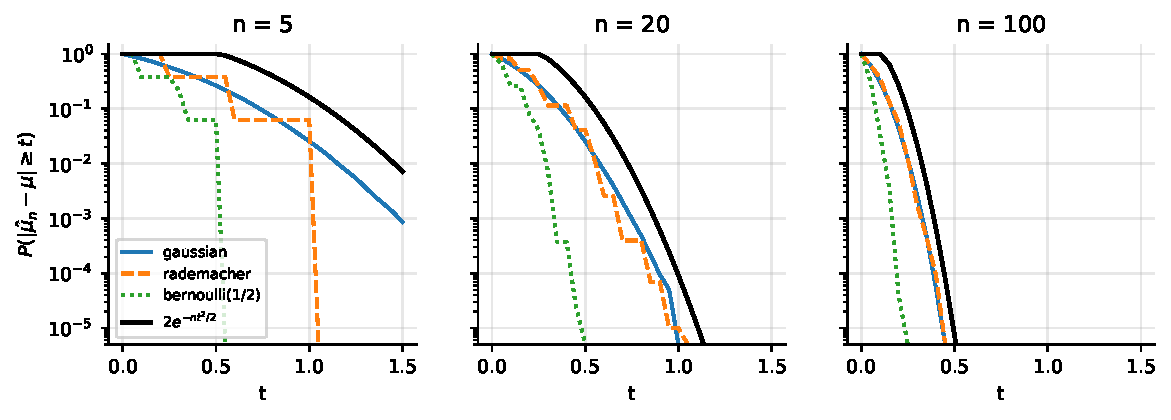
\includegraphics[width=\linewidth]{hoeffding.pdf}
\caption{Empirical tail probabilities (coloured) and the bound $2e^{-nt^2/2}$ (black).}
\label{fig:hoeffding}
\end{figure}

\subsection{(b) Phase-1 regret}

Table~\ref{tab:ucb} and Figure~\ref{fig:ucb} report the phase-1 regret of the UCB rule for $\tau_1\in\{10^3,3\cdot10^3,10^4,3\cdot10^4\}$ and $\Delta\in\{0.1,0.2,0.3,0.5\}$ (means $0.5\pm\Delta/2$). None of the $3{,}200$ runs exceeds bound \eqref{eq:ucb_bound}; the largest regret is $47\%$ of the bound. For $\Delta=0.1$ and $\tau_1\le10^4$ the bound is the trivial $H\Delta$, because $8L_H/\Delta^2$ exceeds $H$. The product $\Delta R(1{:}\tau_1)$ grows linearly in $\log\tau_1$ (right panel), with slope $7.5$--$9.8$ against $8\log(4H^3)/\log H\approx25$ in the bound: the rate $O(\log\tau_1/\Delta)$ is visible, and the constant of the analysis is conservative by a factor of $2.5$ to $3$.

\begin{table}[H]
\centering
\small
\caption{Phase-1 pseudo-regret over 200 runs and the high-probability bound \eqref{eq:ucb_bound} with $\delta=\tau_1^{-2}$.}
\label{tab:ucb}
\begin{tabular}{rrrrrrrr}
\toprule
$\tau_1$ & $\Delta$ & mean & 95\% quantile & max & bound \eqref{eq:ucb_bound} & max $N_j(\tau_1)$ & $1+8L_H/\Delta^2$ \\
\midrule
1,000 & 0.1 & 34.3 & 41.6 & 47.2 & 100.0 & 472 & 17,689 \\
1,000 & 0.3 & 47.3 & 59.1 & 67.2 & 300.0 & 224 & 1,966 \\
1,000 & 0.5 & 43.3 & 53.0 & 60.0 & 354.3 & 120 & 709 \\
10,000 & 0.1 & 171.5 & 211.9 & 251.9 & 1000.0 & 2,519 & 23,215 \\
10,000 & 0.3 & 120.3 & 148.9 & 179.1 & 774.1 & 597 & 2,580 \\
10,000 & 0.5 & 88.5 & 106.0 & 115.5 & 464.8 & 231 & 930 \\
30,000 & 0.1 & 291.0 & 356.5 & 392.3 & 2585.2 & 3,923 & 25,852 \\
30,000 & 0.3 & 157.3 & 189.0 & 234.9 & 862.0 & 783 & 2,873 \\
30,000 & 0.5 & 107.8 & 126.5 & 140.5 & 517.5 & 281 & 1,035 \\
\bottomrule
\end{tabular}
\end{table}

\begin{figure}[H]
\centering
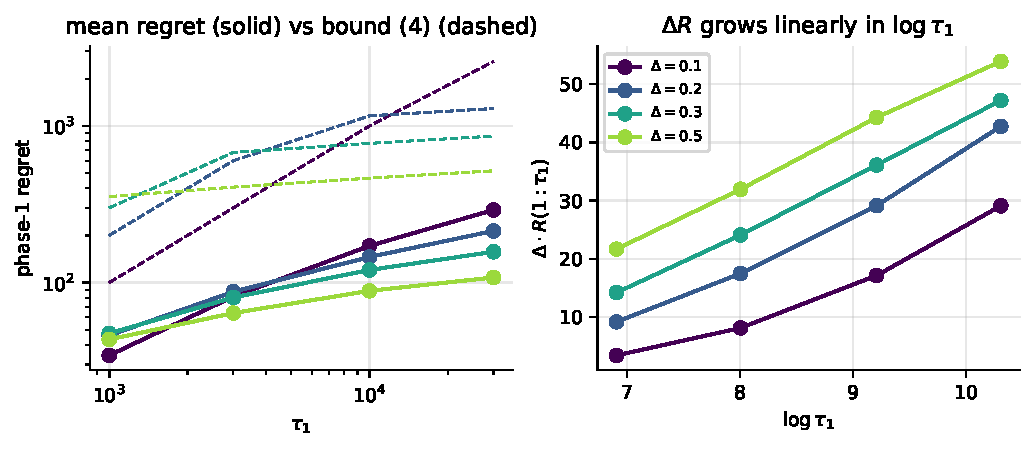
\includegraphics[width=0.9\linewidth]{ucb_phase1.pdf}
\caption{Left: mean phase-1 regret (solid) and bound \eqref{eq:ucb_bound} (dashed). Right: $\Delta\cdot R(1{:}\tau_1)$ against $\log\tau_1$.}
\label{fig:ucb}
\end{figure}

\subsection{(c)(i)--(ii) Window error bounds}

To test \eqref{eq:phase2} and \eqref{eq:phase3} independently of the selection rule, both arms are pulled alternately in scenario S1, so both windows mix samples across both change points. With $\delta=0.05$ and $w\in\{200,1000,3000\}$, no run violates the simultaneous bounds at any round after $\tau_1$ (0 of 200 runs for each $w$); the largest ratio of error to bound is $0.70$, $0.82$ and $0.89$ respectively. The mixing bias computed from the window composition never exceeds the bias terms of \eqref{eq:phase2} and \eqref{eq:phase3} (largest excess $5\times10^{-8}$, single-precision rounding). Figure~\ref{fig:estimation} shows the decomposition: after each change the bias of arm~1 decays linearly in the number of fresh pulls, as in \eqref{eq:alpha}, and reaches zero after $w$ post-change pulls; arm~2 has no bias in phase~2 and a small one after $\tau_2$, where its jump is only $J_{2,2}=0.05$. A longer window lowers the sampling term but stretches the period of bias in proportion to $w$.

\begin{figure}[H]
\centering
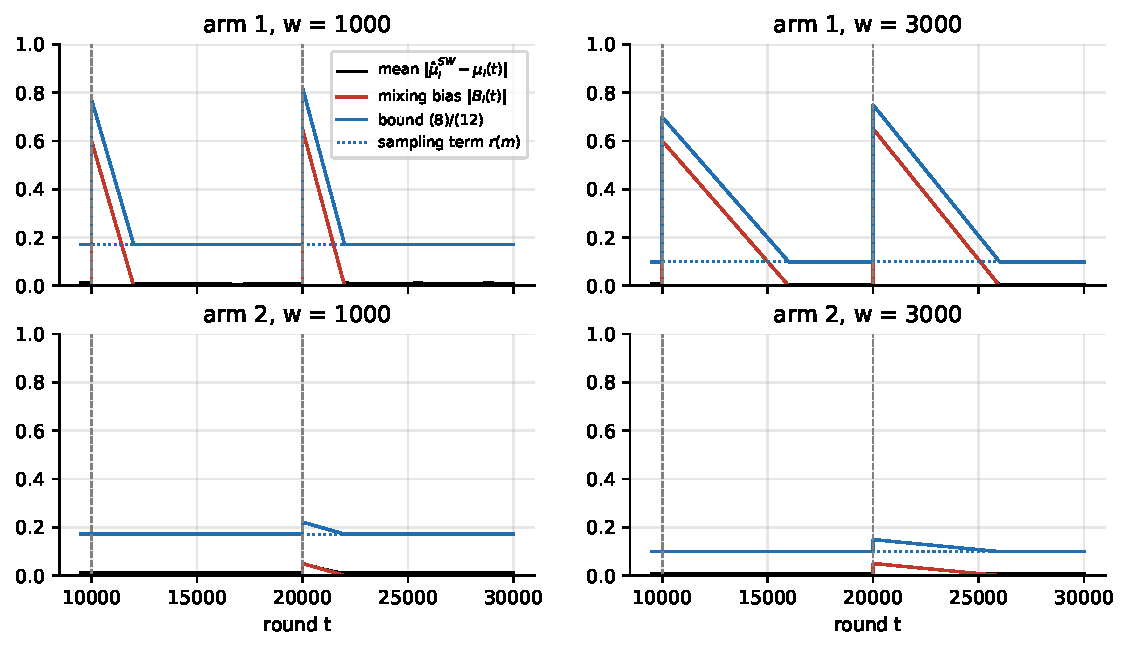
\includegraphics[width=0.95\linewidth]{estimation_bounds.pdf}
\caption{Scenario S1 with alternating pulls: mean absolute error of the window estimate, mixing bias, and the bounds \eqref{eq:phase2}/\eqref{eq:phase3} averaged over 200 runs.}
\label{fig:estimation}
\end{figure}

\subsection{(c)(iii) One window for both change points}

Figure~\ref{fig:window} and Table~\ref{tab:window} report the regret in phases~2 and~3 as a function of $w$. The vertical dotted lines mark the sufficient window $32L_T/g^2$ of \eqref{eq:wprec} ($7{,}824$ for $g=0.3$, $1{,}956$ for $g=0.6$; $70{,}413$ for $g=0.1$ lies outside the plot).

\begin{figure}[H]
\centering
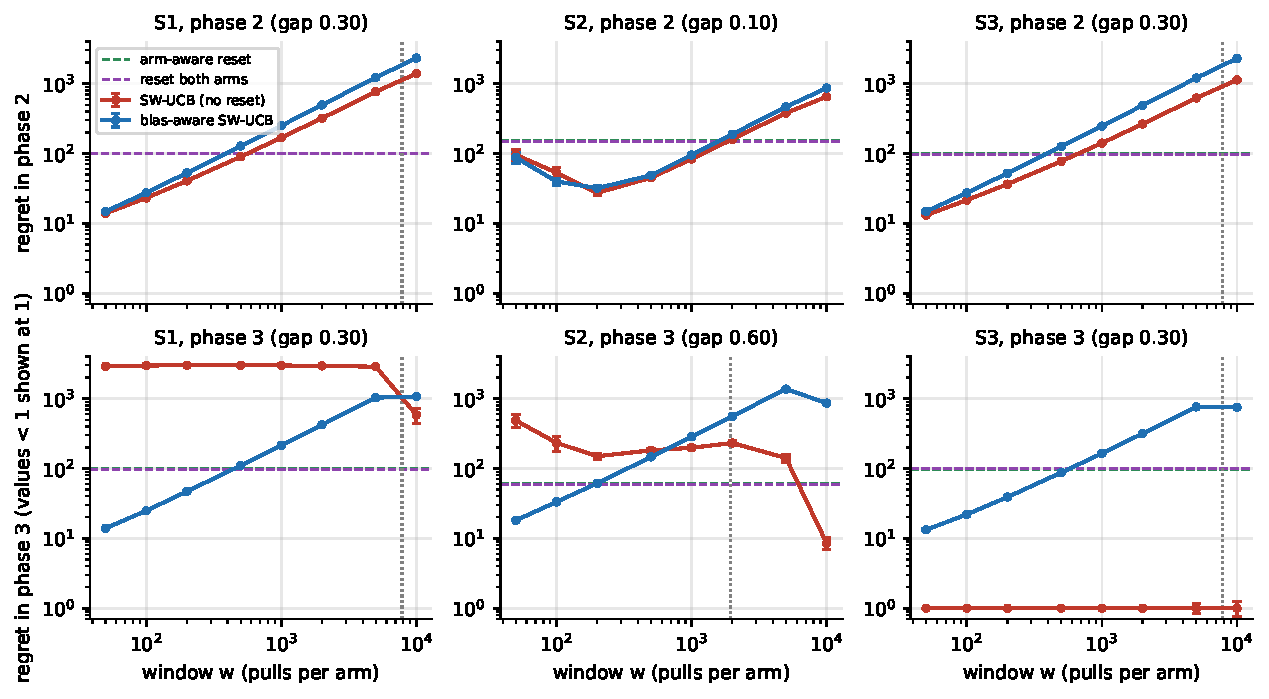
\includegraphics[width=\linewidth]{window_sweep.pdf}
\caption{Regret in phase 2 (top) and phase 3 (bottom) against the window size; dashed lines are the reset variants; 95\% confidence intervals over 200 runs.}
\label{fig:window}
\end{figure}

\begin{table}[H]
\centering
\small
\caption{Best window and regret per phase (mean over 200 runs). For the reset variants the window is unlimited.}
\label{tab:window}
\begin{tabular}{llrrrr}
\toprule
 & & \multicolumn{2}{c}{Phase 2} & \multicolumn{2}{c}{Phase 3} \\
\cmidrule(lr){3-4}\cmidrule(lr){5-6}
Scenario & Policy & best $w$ & regret & best $w$ & regret \\
\midrule
S1 & SW-UCB & 50 & 13.9 & 10,000 & 586.2 \\
 & bias-aware SW-UCB & 50 & 14.8 & 50 & 14.0 \\
 & arm-aware reset & -- & 98.8 & -- & 99.2 \\
\midrule
S2 & SW-UCB & 200 & 27.4 & 10,000 & 8.5 \\
 & bias-aware SW-UCB & 200 & 31.9 & 50 & 18.1 \\
 & arm-aware reset & -- & 154.2 & -- & 60.0 \\
\midrule
S3 & SW-UCB & 50 & 13.1 & any & 0.0 \\
 & bias-aware SW-UCB & 50 & 14.8 & 50 & 13.3 \\
 & arm-aware reset & -- & 100.5 & -- & 96.7 \\
\bottomrule
\end{tabular}
\end{table}

Five observations follow.

\begin{enumerate}
\item \textbf{The window mechanism alone does not guarantee fresh samples.} In S1 and S2 the best arm after $\tau_2$ is arm~1, which was rarely pulled in phase~2. Its window is full of phase-2 observations and does not change while the arm is not selected, so plain SW-UCB keeps the stale ranking: in S1 it pays about $3{,}000$, i.e.\ the full gap in almost every round of phase~3, for every $w\le5{,}000$. This is the requirement stated at the end of part~(c)(iii), and it is not a matter of choosing $w$.
\item \textbf{The confidence radius does not explore when both windows are full.} Once both windows hold $w$ observations, the two radii $r(w)$ are equal and cancel in the comparison of indices, so the rule reduces to comparing window means. Exploration of an unselected arm therefore has to come from elsewhere. The stale-fraction bonus provides it: it is largest for an arm whose window predates its own change, and it vanishes after $w$ fresh pulls. With this bonus the regret in S1 falls from $2{,}907$ to $14$ in phase~3 at $w=50$.
\item \textbf{The sufficient window of \eqref{eq:wprec} is very conservative.} Because the comparison is between window means, the relevant precision is that of the means themselves, of order $\sqrt{\mathrm{Var}/w}$, not the union-bound radius $\sqrt{2L_T/w}$ with $L_T\approx22$. The best windows are $50$--$200$ pulls, one to two orders of magnitude below $32L_T/g^2$, and beyond them regret grows almost linearly in $w$, as the renewal cost \eqref{eq:renewal} predicts.
\item \textbf{Whether one window suffices depends on the gaps.} In S1, where the phase-2 and phase-3 gaps are equal, $w=50$ is best in both phases. In S2 the bias-aware policy is best at $w=200$ in phase~2 (gap $0.1$) and at $w=50$ in phase~3 (gap $0.6$); a common window loses either about $55$ in phase~2 ($w=50$: $87.6$ against $31.9$) or $43$ in phase~3 ($w=200$: $61.2$ against $18.1$). The small gap needs averaging, the large one fast renewal, which is the conflict described in part~(c)(iii).
\item \textbf{A two-arm shift need not be harder.} In S3 both arms move by the same amount and the ranking is unchanged. The stale biases of the two windows have the same sign, and plain SW-UCB has zero regret in phase~3 for every window. The bias-aware policy explores arm~1 because its window is stale, and pays $13$--$761$ for information that is not needed. This is the cancellation described in part~(c)(iii): the jump directions matter, not only the number of arms that change.
\end{enumerate}

The two reset variants have nearly the same regret in all scenarios (within $6$ in every phase). Keeping arm~2's history at $\tau_1$ is worth little here because arm~2 was the worse arm in phase~1 and has few samples to keep. Resets also restart the conservative UCB radius, so their regret ($59$--$154$ per phase) exceeds that of the bias-aware window with a small $w$.

\subsection{(d) Laplace noise}

\paragraph{Coverage of the confidence radius.} Figure~\ref{fig:coverage} compares three radii for means of $n$ Bernoulli$(1/2)$ rewards with added $\mathrm{Laplace}(0,b)$ noise ($4\times10^5$ samples per point): the noise-free radius of part~(a), a radius that only inflates the variance proxy to $1+2b^2$, and the full radius \eqref{eq:rb}. The noise-free radius fails as soon as the noise is non-negligible: at $b=1$ its miscoverage is $1.4$ times $\delta=0.05$ and $10$--$23$ times $\delta=10^{-3}$; at $b=2$ it reaches $174$ times $\delta=10^{-3}$. The variance-only radius is adequate at $\delta=0.05$ but fails in the tail, at $\delta=10^{-3}$ for single observations ($1.3\delta$ for $b=1$, $3.1\delta$ for $b=2$) and for $n=2$ at $b=2$ ($1.4\delta$), because the Laplace distribution is not sub-Gaussian. The full radius \eqref{eq:rb} is valid in all cases, with miscoverage at most $0.04\delta$. This confirms the remark after \eqref{eq:rb}: the linear term $b\log(2/\delta)/n$ is needed.

\begin{figure}[H]
\centering
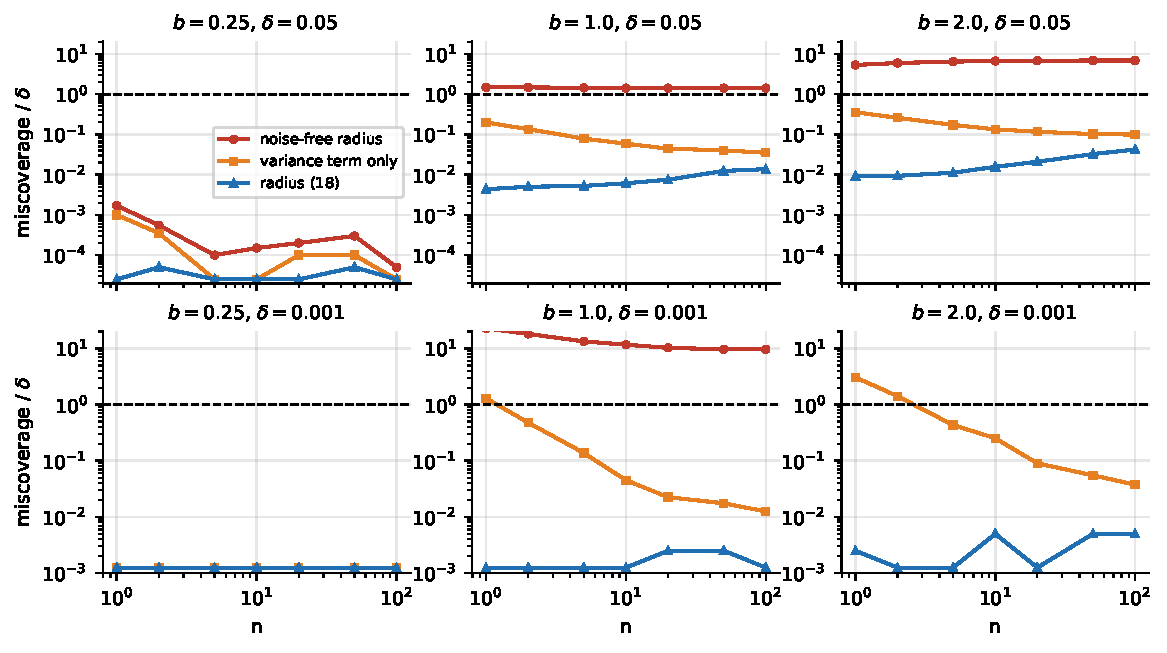
\includegraphics[width=\linewidth]{noise_coverage.pdf}
\caption{Miscoverage divided by $\delta$ (values below the Monte Carlo resolution are shown at the floor); the dashed line is the nominal level.}
\label{fig:coverage}
\end{figure}

\paragraph{Noise shifts the best window upward.} Figure~\ref{fig:noisewindow} repeats the window sweep of scenario S1 for the bias-aware policy with a constant scale $b\in\{0,0.25,0.5,1\}$ and the noisy radius \eqref{eq:noisy_sw}. The window that minimizes the regret after $\tau_1$ grows with the noise: $w=50$ for $b\le0.25$, $100$ for $b=0.5$ and $200$ for $b=1$, where the total regret after $\tau_1$ is $29$, $36$, $70$ and $174$ respectively. Small windows suffer most from the noise ($w=50$: $15\to225$ in phase~2 as $b$ goes from $0$ to $1$), while for $w\ge1{,}000$ the renewal cost dominates and the curves coincide. This is the direction predicted by \eqref{eq:wnoise}: noisier observations require more averaging, at the price of slower renewal.

\begin{figure}[H]
\centering
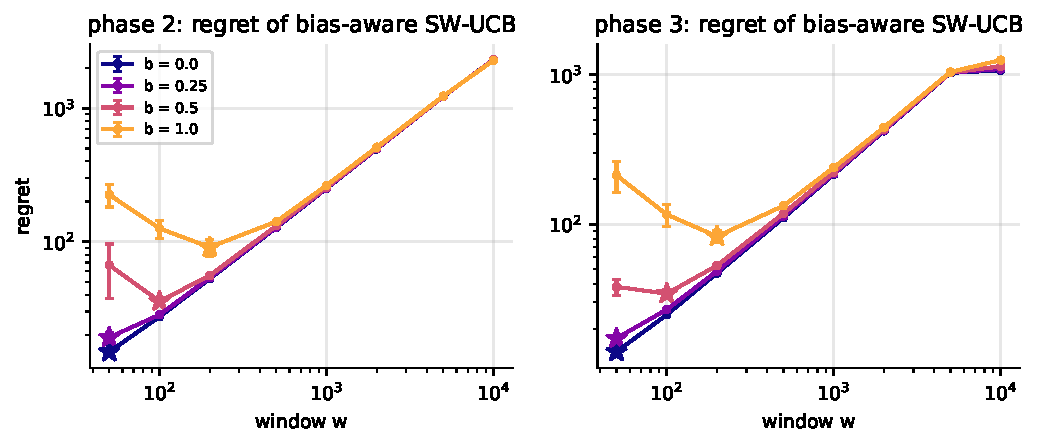
\includegraphics[width=0.9\linewidth]{noise_window.pdf}
\caption{Scenario S1, bias-aware SW-UCB with constant Laplace scale $b$; stars mark the best window.}
\label{fig:noisewindow}
\end{figure}

\paragraph{Allocating a fixed budget.} With $c=1$ and a total budget $E=2T$, uniform spending gives $b_t=0.5$. Following \eqref{eq:blocks}, the horizon is split into three stable blocks and two recovery blocks of $h=2{,}000$ rounds after $\tau_1$ and $\tau_2$; a share $\rho$ of $E$ is spent in the recovery blocks and the rest is spread over the stable blocks in proportion to their lengths ($\rho=2h/T\approx0.13$ is uniform spending). The policy is the bias-aware window with the time-varying radius \eqref{eq:noisy_sw_tv}. Figure~\ref{fig:budget} shows the regret after $\tau_1$ relative to uniform spending. Moderate concentration helps every window: at $\rho=0.25$ (recovery scale $0.27$, stable scale $0.58$) the regret drops by $2.0\%$, $2.5\%$ and $1.6\%$ for $w=300$, $1{,}000$ and $3{,}000$. Stronger concentration helps only the longest window ($-7.1\%$ at $\rho=0.7$ for $w=3{,}000$) and hurts the shorter ones ($+9.6\%$ for $w=300$), whose windows consist mostly of stable-block observations with scale up to $1.44$. This matches the last paragraph of part~(d): budget concentrated around the changes must be balanced against the accuracy of the stable blocks, and the balance depends on $w$. The effects are small in this scenario because the gaps are large compared with the noise; they would grow with smaller budgets or gaps.

\begin{figure}[H]
\centering
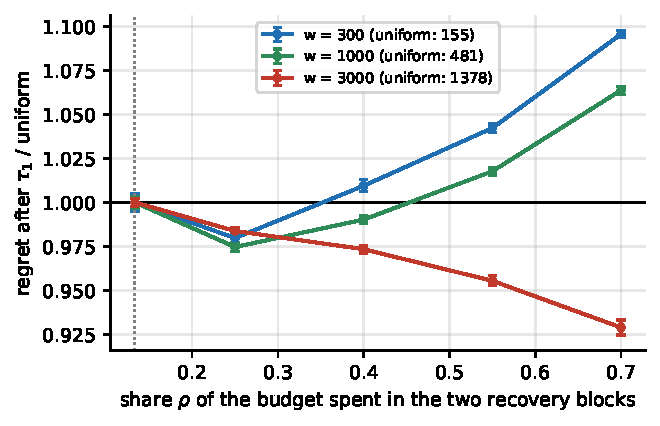
\includegraphics[width=0.6\linewidth]{budget_allocation.pdf}
\caption{Regret after $\tau_1$ relative to uniform spending, as a function of the share of the budget spent in the recovery blocks (dotted line: uniform). 95\% confidence intervals over 200 runs.}
\label{fig:budget}
\end{figure}

\subsection{Summary}

The simulations confirm every bound of the written solution: the Hoeffding bound, the phase-1 regret bound (never exceeded in $3{,}200$ runs, conservative by a factor of $2.5$ to $3$ in its constant), the window error bounds across both change points, and the Laplace confidence radius, whose linear term is needed in the tail. They also sharpen the discussion of part~(c)(iii). A sliding window over pulls must be combined with a mechanism that refreshes stale arms; a bonus equal to the stale fraction of the window, applied only to arms whose mean has changed, does this and uses the asymmetry between the two change points. With that mechanism, a single window suffices when the post-change gaps are comparable but not when they differ, and a common shift of both arms costs nothing to a policy that does not explore. Laplace noise moves the best window upward, and concentrating a fixed budget around the change points helps only up to a point that depends on the window.


\end{document}
